\chapter{Measure Theory in Probability Theory}
\label{ch:measure-theory}

Measure theory \parencites{tao2011introduction}[section 10.5]{bronstein1995taschenbuch} allows to treat both
discrete and continuous probabilities under a common, generalized notation, primarily by the
introduction of integrals over measures.  The basic idea of a measure is to generalize the concept
of a \enquote{volume function} on sets.

A \emph{measure space} is a triple \((\Omega, \mathcal{A}, \mu)\), where
\(\mathcal{A} \subseteq 2^{\Omega}\) is a \(\sigma\)-algebra of \emph{measurable sets} (i.e., closed
under complement, countable union, and countable intersection), and
\(\mu: \mathcal{A} \to \RR \cup \{\infty\}\) is a \(\sigma\)-additive function:
\begin{equation}
  \label{eq:sigma-additivity}
  \mu\left( \bigcup_{k} A_k \right) = \sum_{k} \mu(A_k)
\end{equation}
for all disjoint countable families \((A_k)\) in \(\mathcal{A}\).  Additionally, we require that
\(\mu(\emptyset) = 0\).  The necessity for \(\mathcal{A}\) and \(\mu\) being defined in such an
elaborate way, instead of just taking it as \(2^{\Omega}\), is that for uncountable \(\Omega\), it
is not possible to consistently assign a measure for the complete powerset.  The restriction to
measurable subsets specifically filters out those pathological cases.

In probability theory \parencite{kallenberg2006foundations}, one always operates within a special
measure space called \emph{probability space}.  In a probability space \((\Omega, \mathcal{A}, P)\),
we additionally require that \(P(\Omega) = 1\).  \(\Omega\) is then called the set of
\emph{events}~-- think of all possible outcomes of some experiment. 

A function between measure spaces, or probability spaces in particular, is called \emph{measurable}
when every preimage of a measureable set is measurable.  A \emph{random variable} \(X\) is a
measureable function \((\Omega, \mathcal{A}, P) \to (\Psi, \mathcal{B}, P_X)\) from a probability
space to another one with a \emph{pushforward} \(P_X\), such that
\begin{equation}
  \label{eq:pushforward}
  P_X(B) = P(X^{-1}(B))
\end{equation}
for all \(B \in \mathcal{B}\).  The introduction of random variables allows to consistently convert
set-theoretic operations on events into \enquote{numerical} ones: think of assigning to each outcome
of a coin throw a number in \(\{1, 2\}\), or to each measurement of some height a value in
\(\RR^{+}\).  In practice, this allows us to forget about the underlying event space and think
solely in terms of the values in the domain of the random variable, with notation like
\begin{equation}
  \label{eq:prob-notation}
  \Prob{\alpha(X)} = P(\{\omega \in \Omega \mid \alpha(X(\omega))\})
\end{equation}
where \(\alpha\) is an arbitrary predicate defining a set in the domain of \(X\).

In such a setting, it might the case that there exist some \emph{base measure} \(\mu\), such that
probability evaluation can be expressed as integral over some \emph{density} with respect to \(\mu\):
\begin{equation}
  \label{eq:measure-integral}
  \Prob{X \in A} = \int_{A} \prob[X]{x} \dif\mu(x),
\end{equation}
for all \(P_X\)-measureable sets \(A\), or in differential notation
\begin{equation}
  \label{eq:measure-differential}
  \Prob{X \in \dif x} = \prob[X]{x} \dif\mu(x).
\end{equation}
In this case \(P_X\) is said to be \emph{absolutely continuous} with respect to \(\mu\), written
\(P_X \ll \mu\).  This statement is equivalent to the existence of a \emph{Radon-Nikodym derivative}
\begin{equation}
  \label{eq:radon-nikodym}
  \frac{\dif P_{X}}{\dif \mu} = p_{X}.
\end{equation}
For discrete values, a density always exists with respect to the counting measure, and the random
variable is also called discrete.  For finite-dimensional continuous values, when a density exists
with respect the Lebesgue measure, we speak of a continuous random variable. 




\chapter{Details of Automatic Differentiation}
\label{ch:ad-details}

The standard reference for AD is \textcite{griewank2008evaluating}.  \textcite{baydin2018automatic}
gives a comprehensive survey including a comparison of state-of-the-art implementations.  There are
many works on the formalization of AD; see, for example, \textcite{abadi2020simple},
\textcite{vytiniotis2019differentiable}, \textcite{wang2019demystifying},
\textcite{sajovic2016operational}, or \textcite{elliott2018simple}.

To understand how AD works, let us first start with the mathematics.  What is a derivative, really?
When we talk about gradients, which is what we really need in a gradient algorithm, this is usually
a rather informal term for \enquote{the vector of partial derivatives}, which then points into an
ascent direction.  This is however not the most natural form to work with in a compositional
approach.  Instead of starting with a limit of tangent slopes, more insight is provided by viewing
derivatives as best-approximating linear operators.  One of the most general definitions is provided
through the \emph{Fréchet derivative} \parencite[p. 463]{bronstein1995taschenbuch}, essentially a
generalization of the total differential\footnote{I prefer thinking in terms of the Fréchet
  derivative, since it makes explicit the fact that derivatives are operators, and provides enough
  flexibility while still being intuitive.  Different abstractions are possible, though.}.  Let
\(X\) and \(Y\) be normed spaces.  A function \(f: U \subseteq X \to Y\) is Fréchet differentiable
at a point \(x \in U\) if there exists a bounded linear operator \(A: X \to Y\) such that
\begin{equation}
  \label{eq:frechet}
  \lim_{\enVert{\Delta}_X \to 0} \frac{\enVert{f(x + \Delta) - f(x) -
      A(\Delta)}_Y}{\enVert{\Delta}_X} = 0.
\end{equation}
When such an \(A\) does exist, it is unique, and we may call it \emph{the} derivative of \(f\) at
\(x\), writing \(\Dif f(x) = A\).  When the derivative exists for all \(x\), we can use \(\Dif\) as
a well-defined higher-order function on its own; we will assume this in the following.\footnote{In
  in practical cases, functions are often only piecewise differentiable due to branches, failing
  this definition on a countable set of points.  Fortunately, the formalism of AD remains the same
  under weaker notions of differentiability.  Additionally, such points usually behave well enough
  to admit a subdifferential, from which we can just choose an arbitrary subgradient; this does not
  necessary lead to a descent direction, but still allows minimization under reasonable conditions
  \parencites[see][section 6.1]{pock2017convex}[][chapter
  14]{griewank2008evaluating}{abadi2020simple}.}

The important fact here is that \(\Dif f(x)\) is still a function: specifically, a linear function
approximating how \(f\) reacts to an input perturbation, \(\Delta\), around \(x\).  Or, in other
words:
\begin{equation}
  f(x + \Delta) = f(x) + \Dif f(x)(\Delta) + o\left(\enVert{\Delta}\right).
\end{equation}
This fact allows one to propagate differential values through composed functions, by the chain rule,
which we write in the following compositional form:
\begin{equation}
  \Dif(\phi \circ \psi)(x) = \Dif\phi(\psi(x)) \circ \Dif\psi(x).
\end{equation}
for differentiable functions \(\phi\) and \(\psi\).  In the one-dimensional case, we simply have
\begin{equation}
  \Dif \phi(x) = \Delta \mapsto \partial_1 \phi(x) \, \Delta,
\end{equation}
where \(\partial_1 \phi(x)\) denotes the standard \enquote{primitive} derivative, since linear maps
are exactly multiplications by a scalar.  Therefore, we can recover the chain rule
\begin{equation}
  \begin{aligned}
    \Dif(\phi \circ \psi)(x)(\Delta) &=
    \left( \Dif\phi(\psi(x)) \circ \Dif\psi(x) \right)(\Delta) \\
    % &= \Dif\phi(\psi(x))\left( \Dif\psi(x)(\Delta) \right) \\
    % &= \Dif\phi(\psi(x))\left( \partial_1 \psi(x) \, \Delta \right) \\
    % &= \partial_1\phi(\psi(x)) \, \partial_1 \psi(x) \, \Delta \\
    &= \left( \partial_1\phi(\psi(x)) \, \partial_1 \psi(x) \right) \, \Delta,
  \end{aligned}
\end{equation}
as we know it from calculus.  Here, the product in the resulting expression arises from the fact
that we propagated through \(\partial_1 \psi(x) \Delta\) as the input value of
\(\Dif\phi(\psi(x))\).  It is, however, remarkable that this formula is not entirely compositional:
to construct \(\Dif(\phi \circ \psi)\), it is not only necessary to know \(\Dif\phi\) and
\(\Dif\psi\), but also \(\psi\) \parencite{elliott2018simple}.  Still, this is not as bad as it may
seem: as I will now explain, AD algorithms evaluate both \((\phi \circ \psi)(x)\) and
\(\Dif(\phi \circ \psi)(x)\) at once, in lockstep fashion, so that the intermediate values of the
former can be reused in calculation of the latter.

Consider the specific case of \(f(x, y) = sin(x) - y\). For simpler notation, let
\(g = (x, y) \mapsto x - y\) replace the infix subtraction operator, with a derivative of
\(\Dif g(x)(\Delta_1, \Delta_2) = \Delta_1 - \Delta_2\), a linear function of two arguments.  By
composition, we have:
\begin{equation}
  \begin{aligned}
    \Dif f(x, y) &= \Dif(g \circ (\sin \otimes \ident))(x, y) \\
    &= \Dif g\left( (\sin \otimes \ident)(x, y) \right) \circ \Dif(\sin \otimes \ident)(x, y) \\
    % &= \left( (\Delta_1, \Delta_2) \mapsto \Delta_1 - \Delta_2 \right) \circ \left( \Dif\sin(x)
      % \otimes \Dif \ident(y) \right) \\
    % &= (\Delta_1, \Delta_2) \mapsto \partial_1\sin(x) \, \Delta_1 - 1 \Delta_2 \\
    &= (\Delta_1, \Delta_2) \mapsto \cos(x) \, \Delta_1 - \Delta_2
  \end{aligned}
\end{equation}
(where \(\ident\) is the identity function, and
\((\phi \otimes \psi)(\alpha, \beta) = (\phi(\alpha), \psi(\beta))\) defines product morphisms).  In
order to calculate this algorithmically, let us expand the computation of \(f\) into a sequence of
intermediate, primitive calculations, as we would have in a programmatical representation:
\begin{equation}
  \label{eq:ad-primal}
  \begin{aligned}
    x &= \operatorname{?}, \\
    y &= \operatorname{?}, \\
    z &= \sin(x), \\
    \Omega &= g(z, y).
  \end{aligned}
\end{equation}
We have given the final result the name \(\Omega\), and and introduced an intermediate value \(z\).
This is known as the \emph{forward}, or \emph{primal} function in AD terminology.  The relations of
these values can be expressed as the black computation graph in figure~\ref{fig:comp-graph-fw}.
Following the graph, or equivalently, following the equations in ~\eqref{eq:ad-primal}, the
composition of the derivative operators can be built up incrementally, as shown in the blue part of
that figure, by calculating the following \emph{tangent values}:
\begin{equation}
  \label{eq:ad-forward}
  \begin{aligned}
    \dot{x} &= \Delta_1, \\
    \dot{y} &= \Delta_2, \\
    \dot{z} &= \Dif\sin(x)(\dot{x}) \\
    &= \cos(x) \, \Delta_1, \\
    \dot{\Omega} &= \Dif g(z, y)(\dot{z}, \dot{y}) \\
    &= \cos(x) \, \Delta_1 - \Delta_2.
  \end{aligned}
\end{equation}
The tangent values of input variables \(x\) and \(y\) become the input perturbations \(\Delta_1\),
\(\Delta_2\).  For every subsequent tangent value, we apply the derivative at the corresponding
primal variable (depending on the primal parents) to the tangent values of the parents~-- this way,
the composition of the derivative operators follows the chain rule.  This algorithm, called
\emph{forward-mode AD}, can now be applied practically not only on symbolic functions, but on
programs, by always jointly computing \((v, \dot{v})\) for every variable \(v\), given its parents
in the graph.  This requires a form of non-standard execution.

\begin{figure}[t]
  \centering
  \subbottom[Forward mode.\label{fig:comp-graph-fw}]{%
    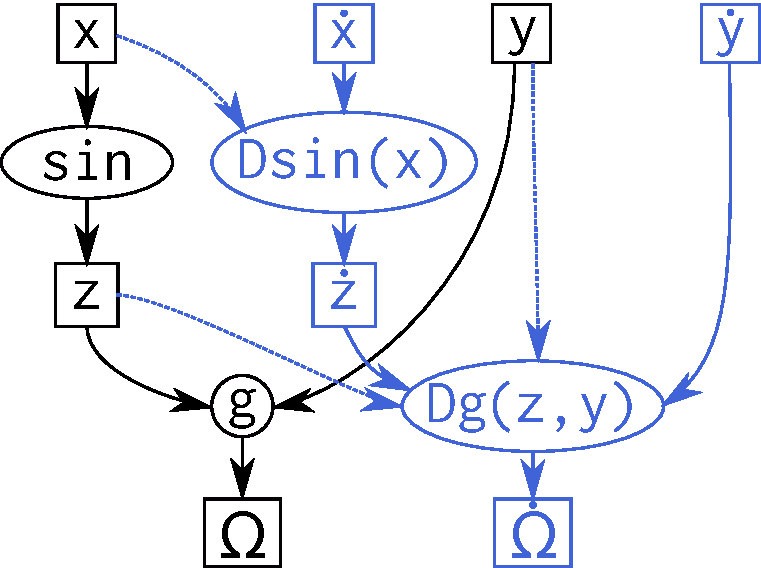
\includegraphics[]{figures/comp-graph}}
  \qquad
  \subbottom[Backward mode.\label{fig:comp-graph-bw}]{%
    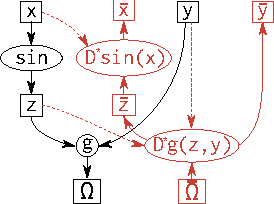
\includegraphics[]{figures/comp-graph-backward}}
  \caption{Computation graph and intermediate expressions of the expression \protect\jlinl{g(sin(x),
      y)}, together with the derivative graphs in forward- and backward mode.  Dashed arrows
    indicate re-use of primal values in the derivative graph.}
  \label{fig:comp-graph-2}
\end{figure}

\newthought{Recovering the full gradient} of a multivariate function
\(\phi: U \subseteq \RR^N \to \RR\) (which is generally the form of loss functions for parametric
models) requires to evaluate \(\Dif \phi(x)\) \(N\) times, however.  This is because individual
partial derivatives can only be extracted from \(\Dif \phi(x)\) by calculating the sensitivities to
unit input perturbations in coordinate directions, for each of the input variables:
\begin{equation}
  \nabla \phi(x) = \begin{pmatrix}
    \Dif \phi(x)(1, 0, \ldots, 0)  \\
    \vdots \\
    \Dif \phi(x)(0, \ldots, 0, 1)
  \end{pmatrix} = \begin{pmatrix}
    \partial_1 \phi(x) \\
    \vdots \\
    \partial_N \phi(x)
  \end{pmatrix},
\end{equation}
which is really a special case of taking directional derivatives (which can be recovered generally
by application of the differential to any vector with unit norm.)

In order to overcome the increase of complexity with the number of input dimensions, we can
reformulate the compositional equation.  Let us introduce \(\CoDif \phi(x)\), the \emph{adjoint
  operator} of \(\Dif \phi(x)\), whose defining property is that \enquote{inverts} the order of the
perturbation application: instead of calculating a primal sensitivity with respect to an input
perturbation (\(\Delta\)), it maps a linear output perturbation (\(\mathfrak{d}\)) to an operator
that applies this to the primal sensitivity:
\begin{equation}
  \CoDif \phi(x)(\mathfrak{d}) = \Delta \mapsto \mathfrak{d}(\Dif \phi(x)(\Delta)).
\end{equation}
The adjoint differential is therefore an object of the double dual space.  This becomes more
readable when we fix a basis to represent the derivative.  Doing so, in the finite-dimensional case,
the derivative \(\Dif \phi(x)\) is the Jacobian matrix at \(x\), \(J_{\phi}(x)\).  In this setting,
forward-mode AD is simply an efficient way to calculate the \emph{Jacobian-vector product}
\(J_{\phi}(x) \Delta\), or equivalently the total derivative for a fixed perturbation, avoiding full
matrix multiplication~-- which is the reason we have to apply it to the basis vectors to get back
the gradient.  Backward mode, on the other hand, calculates the product of the Jacobian with the
operator that should be applied to the result, but does not yet apply it to the input
perturbation~-- therefore, it returns a matrix:
\begin{equation}
  \begin{aligned}
    \mathfrak{d} (\Dif \phi(x)(\Delta)) &= \transpose{d} J_{\phi}(x) \Delta \\
    &= \transpose{\left( \transpose{J_{\phi}(x)} d \right)} \Delta \\
    &= \CoDif \phi(x)(\mathfrak{d})(\Delta),
  \end{aligned}
\end{equation}
where we assume \(\mathfrak{d}\) to be represented by the co-vector \(\transpose{d}\).  Since the
unapplied \(\CoDif \phi(x)(\mathfrak{d})\) is itself an object in the dual space, it is also
represented as a co-vector~-- and in fact, nothing else than a transformation of the transposed
Jacobian, or a \emph{vector-Jacobian product}.  Recovering the gradient of a loss function then
reduces to evaluating it at a constant scalar output perturbation of \(1\), which is equivalent to
the application of the primal differential to the matrix of basis vectors.

Note that due to this relation to the transpose, the adjoint operator inverses the order of
composition in the chain rule:
\begin{equation}
  \begin{aligned}
    \CoDif (\phi \circ \psi)(x)(\mathfrak{d}) &= \transpose{d} J_{\phi}(\psi(x)) J_{\psi}(x) \\
    &=  \transpose{\left( \transpose{J_{\psi}(x)} \transpose{J_{\phi}(\psi(x))} d \right)} \\
    &= \left( \CoDif\psi(x) \circ \CoDif\phi(\psi(x)) \right)(\mathfrak{d}).
  \end{aligned}
\end{equation}
For our example function \(f\), this gives the same structural form of the result as the forward
mode~-- only that now, the value is a vector:
\begin{equation}
  \begin{aligned}
    \CoDif f(x, y) &= \CoDif (g \circ (\sin \otimes \ident))(x, y) \\
    &= \CoDif(\sin \otimes \ident) \circ \CoDif g((\sin \otimes \ident)(x, y)) \\
    % &= (\CoDif\sin \otimes \CoDif\ident) \circ (\delta \mapsto \transpose{[\delta, -\delta]}) \\
    % &= (\partial_1 \sin(x) \otimes 1) \circ (\delta \mapsto \transpose{[\delta, -\delta]}) \\
    % &= \delta \mapsto \transpose{[\partial_1\sin(x)\delta, -1 \delta]} \\
    &= \delta \mapsto \transpose{[\cos(x)\delta, -\delta]}.
  \end{aligned}
\end{equation}
In this form, starting with an output perturbation \(\delta = 1\), we get back the gradient tuple
through just one evaluation.  Incidentally, this is nothing else than the back-propagation
\enquote{trick} \parencite{bishop2006pattern}!  Furthermore, applying this result to
\([\Delta_1, \Delta_2]\) gives back the linear combination of the forward mode result.

In programmatic terms, we can proceed similar to above, only this time introducing \emph{adjoint}
intermediate values \(\bar{v}\).  For the values in equation~\eqref{eq:ad-primal}, we get
\begin{equation}
  \label{eq:ad-backward}
  \begin{aligned}
    \bar{x} &= \bar{z}_2 = -\delta, \\
    \bar{y} &= \CoDif\sin(x) \, \bar{z}_1 \\
    &= \cos(x) \, \delta\\
    \bar{z} &= \CoDif g(x, y)(\bar{\Omega}) \\
    &= [\delta, -\delta] \\
    \bar{\Omega} &= \delta,
  \end{aligned}
\end{equation}
which is displayed in the red graph in \ref{fig:comp-graph-bw}.  Note that now, the back-propagated
values can not be computed in parallel with forward evaluation; hence the equations are stated in
reverse order.  Instead, the intermediate primal values have to be remembered and reused in a
second, backward pass.

Finally, it has to be noted that the two described modes of automatic differentiation are only two
extremes of a spectrum.  Forward and backward calculations can really be interleaved in arbitrary
order, just as it is possible to multiply Jacobians and their transposes in different order.  One
frequent use case of this \emph{mixed-mode AD} is when loss functions, differentiated using backward
mode, contain broadcasting functions; for example, nonlinearities within neural networks.  These
have a type of \(\RR^N \to \RR^N\), but only involve a linear number of operations, so forward mode
pays off\footnote{As a rule of thumb in Julia, for \(f: \RR^M \to \RR^N\), forward mode typically
  performs better when \(M \ll N\) or as long as \(M \lessapprox 100\).  This folklore should always
  be confirmed by benchmarking, though.  See
  \url{https://github.com/JuliaDiff/ReverseDiff.jl\#should-i-use-reversediff-or-forwarddiff}.}.
Similar properties hold for second order derivatives: the calculation of Hessians is often fastest
by using forward-over-reverse composed differentiation.  In general, unfortunately, determining the
optimal order of derivative evaluation is hard~-- this so-called \emph{optimal Jacobian
  accumulation} problem is known to be NP-complete \parencite{naumann2007optimal}.

\section{Dual Numbers}
\label{sec:dual-numbers}

Forward mode can be recast in mathematically equivalent form by using dual numbers
\parencite[see][section 3.1.1]{baydin2018automatic}{deakin1966functions}.  These consist of two
parts, similar to complex numbers: \(z = x + y\epsilon\).  However, contrary to the imaginary unit,
the infinitesimal unit \(\epsilon\) vanishes under multiplication with itself: \(\epsilon^2 = 0\).
The consequence of this is that functions can naturally be extended to dual numbers by nonstandard
interpretation as truncated Taylor series:
\begin{equation}
  \phi(x + \epsilon) = \phi(x) + \partial_1\phi(x)\epsilon + \underbrace{\frac{\partial^2_1\phi(x)}{2}\epsilon^2
  + \ldots}_{\epsilon^2 (\ldots) = 0}
\end{equation}
Since the higher order terms vanish, this is exactly the tuple of primal and tangent value that is
calculated during the lockstep evaluation in forward mode:
\begin{equation}
  (z, \dot{z}) = (\phi(x), \Dif\phi(x)(\dot{x})) \quad\Leftrightarrow\quad z + \dot{z}\epsilon = \phi(x + \dot{x}\epsilon).
\end{equation}
The generalization to higher dimensions, as well as higher derivatives in form of hyper-dual numbers
\parencite{fike2012automatic}, follow naturally.





%%% Local Variables: 
%%% TeX-master: "main"
%%% End: